\documentclass[a4paper,12pt]{report}
\usepackage{color}
\usepackage{hyperref}
\hypersetup{
    colorlinks,
    citecolor=black,
    filecolor=black,
    linkcolor=black,
    urlcolor=black
}
\setcounter{secnumdepth}{0}
\setcounter{tocdepth}{3}
\usepackage{graphicx}
\usepackage{epstopdf}
\epstopdfsetup{outdir=./}
\usepackage{amsmath}
\usepackage[table,xcdraw]{xcolor}
\usepackage{amssymb}
\usepackage{listings}
\definecolor{anti-flashwhite}{rgb}{0.95, 0.95, 0.96}
\lstset{
	language=C++,
    basicstyle=\ttfamily,
    keywordstyle=\color{blue}\ttfamily,
    stringstyle=\color{red}\ttfamily,
	commentstyle=\color{green}\ttfamily,
    morecomment=[l][\color{magenta}]{\#},
    backgroundcolor=\color{anti-flashwhite}
}
\begin{document}
\title{
\textbf{Distributed Computing - II: CS5320}\\~\\
\begin{huge}
\textbf{Programming Assignment 2:\\Termination Detection
\\~\\}
\end{huge}
\begin{huge}
\textbf{Assignment Report}
\end{huge}
}
\author{\textbf{Sagar Jain - CS17BTECH11034}\\}
\maketitle
\begin{large}
\tableofcontents
\end{large}
\newpage
\section{Program Design}
\textbf{An important notice, for both the programs is that they may not terminate when all the cells have turned red, in these cases one must restart the execution, this is something inherent to the problem and cannot be avoided.}
\subsection{Spanning Tree Algorithm}
\subsubsection{Cell Struct}
The cell struct represents each node in the distributed network. The following constitutes the cell.
\begin{enumerate}
\item A vector of all the children nodes of the node i.e. \textbf{children}.
\item A boolean array which represents if the tokens were received from a particular node i.e \textbf{tokenReceived}.
\item A boolean which represents if a node has a token or not i.e. \textbf{haveToken}.
\item \textbf{cellColour}, the colour of the cell.
\item \textbf{nodeColour}, the colout of the node, which also ends up becoming the colour of the token which the node sends to its parent.
\item A mutex lock which is used to achieve mutual exclusion every time data of this cell is being accessed i.e \textbf{lock}.
\end{enumerate}
\subsubsection{Cell Process}
This is the function which every cell runs when it is launched, it also launches another process which is used to receive messages from other threads. The following are the main tasks of this function.
\begin{enumerate}
\item Launch the receiving threads.
\item Wait for the listening threads to begin listening before beginning to send messages. This is done using \textbf{pthread\_cond\_wait}.
\item Start sending encoded messages of the colour of the cell (red or blue) to a corresponding number of the neighbours of the cell.
\item After each round of sending messages, check if the cell has received tokens from all the children and if so, if the cell itself is currently blue, if both theses condition are satisfied then send a token of the colour of the node (\textbf{node colour and cell colour are different things}) to the parent.
\item Once a token is sent to the parent, the \textbf{receivedToken} vector has all its entries sent to false as we must wait for all the childrent to send tokens once again before this cell can send a token to its parent,
\end{enumerate}
\subsubsection{Receiver Process}
This function is responsible for handling the receiving of messages from other cells, and taking appropriate action on the receipt of said messages.
The main tasks of this function are highlighted below:
\begin{enumerate}
\item The receiving process first sets up the listening server, and after each server is set up it increments a variable in the critical section, using  a \textbf{pthread\_conditional\_variable} we can broadcast to all the sending threads that they can begin sending messages once the value of this variable is equal to the number of cells.
\item On receiving a message the receiving thread decodes the contents of the message, i.e. the sender id and the encoded digit which signifies the colour of the node cell or the colour of the token. A message can either be one which contains a token or one which contains the colour of the sender.
\item After decoding the contents of the message a given cell, changes or doesn't change its cell colour and/or node colour based on the contents of the received message.
\end{enumerate}
\subsubsection{Miscellaneous}
The following is the message encoding format and meaning:\\
Every message begins with the sender id, this is followed by a delimiting \#, that is followed by one of the following numbers,\\
 1 - White Message\\
 2 - Red Message\\
 3 - Blue Message\\
 4 - White Token\\
 5 - Black Token\\
\subsection{Message Optimal Algorithm}
\subsubsection{Cell Struct}
The cell struct represents each node in the distributed network. The following constitutes the cell.
\begin{enumerate}
\item Vectors \textbf{To} and \textbf{From} which represent the To and From stacks from the algorithm, using two vectors has the advantage that we do not need to encode to and from messages onto the same stack, it also \textbf{makes the search and traversal during stack clean up}.
\item A vector \textbf{colouredLinks}, this keeps track of all the incoming links coloured by the cell. We do not keep a similar vector for outgoing links, this is because of the observation that all outgoing links can be assumed to be coloured as soon as the cell is in DT, this makes the check easier and reduces overhead.
\item A vector of all the children nodes of the node i.e. \textbf{children}.
\item A boolean array which represents if the terminate was received from a particular node i.e \textbf{terminateReceived}.
\item A boolean which represents if a node has sent terminate signal to its parent or not i.e. \textbf{sentTerminate}.
\item A boolean which represents if a node is in DT or not i.e. \textbf{DT}.
\item A boolean which represents if a node has sent warning signal to its neighbours or not i.e. \textbf{sentWarningToNeighbours}.
\item \textbf{cellColour}, the colour of the cell.
\item A mutex lock which is used to achieve mutual exclusion every time data of this cell is being accessed i.e \textbf{lock}.
\end{enumerate}
\subsubsection{Cell Process}
This is the function which every cell runs when it is launched, it also launches another process which is used to receive messages from other threads. The following are the main tasks of this function.
\begin{enumerate}
\item Launch the receiving threads.
\item Wait for the listening threads to begin listening before beginning to send messages. This is done using \textbf{pthread\_cond\_wait}.
\item Start sending encoded messages of the colour of the cell (red or blue) to a corresponding number of the neighbours of the cell.
\item\textbf{On sending a red message to any neighbour, the cell adds the id of the cell to the To vector, this is because this cell will need a response from that cell that it has turned blue.}
\item Every round the cell also checks if it has entered DT, if it has then it checks if it has already sent the warning message to its neighbours, if not it send the warning message to all its neighbours.
\item After each round of sending messages, check if the cell has received terminate from all the children and if so, if the cell itself is currently blue, all links are coloured and if its stack is empty, if all theses condition are satisfied then send a terminate signal to the parent.
\item \textbf{Every iteration, the cell, if blue (i.e. idle) executes the stack clean up routine in which it goes through the from vector and sends all the neighbours in the from vector the remove\_entry message.}
\item \textbf{Terminate signal is only sent once from every child to the parent, this is done using a check if a terminate signal has already been sent within each cell. This helps us keep the algorithm "message optimal"}.
\end{enumerate}
\subsubsection{Receiver Process}
This function is responsible for handling the receiving of messages from other cells, and taking appropriate action on the receipt of said messages.
The main tasks of this function are highlighted below:
\begin{enumerate}
\item The receiving process first sets up the listening server, and after each server is set up it increments a variable in the critical section, using  a \textbf{pthread\_conditional\_variable} we can broadcast to all the sending threads that they can begin sending messages once the value of this variable is equal to the number of cells.
\item On receiving a message the receiving thread decodes the contents of the message, i.e. the sender id and the \textbf{encoded digit which signifies the colour of the node cell or whether it is a warning, terminate or removeEntry message}.
\item After decoding the contents of the message a given cell, changes or doesn't change its cell colour.
\item On receiving a warning message, \textbf{the cell colours the incoming link and also sends a warning message to all its neighbours, we assume that all its outgoing links are now coloured.}
\item On receiving a remove\_entry message the cell removes one instance of the sender ID from the its local \textbf{From list}.
\item On receiving a terminate message, the parent cell notes the fact that this particular child has sent a terminate message and uses this fact later on to send a terminate message it its own parent.
\end{enumerate}
\subsubsection{Miscellaneous}
The following is the message encoding format and meaning:\\
Every message begins with the sender id, this is followed by a delimiting \#, that is followed by one of the following numbers,\\
 1 - White Message\\
 2 - Red Message\\
 3 - Blue Message\\
 4 - Warning Message\\
 5 - Terminate Message\\
 6 - Remove Entry Message\\
\subsubsection{Some Common Patterns}
\begin{enumerate}
\item Conditional variables have been used when threads are waiting for a particular condition to be satisfied. This has been done using the posix pthread utilities i.e. \textbf{pthread\_condition\_variables}, \textbf{pthread\_cond\_broadcast}, etc.
\item \textbf{fprintf} has been used while writing to files since it does not produce errors when multiple processes are writing to the file at the same time.
\item \textbf{pthread\_cancel} has been used since at the end of the termination algorithm as our aim is to simply simulate the detection of termination and following that we just need to exit the program.
\item Condition compilation has been used to avoid debug output during actual testing of the code, this has been done using \textbf{ifndef}, and the debug output will be disabled by default.
\item The port numbers of servers are selected in the following fashion. Server i has a port number of the form 50000 + i or 55000 + i for the first and second program respectively.
\end{enumerate}
\section{Program Output}
\subsection{Spanning Tree Algorithm}
Example Output for the Spanning Tree Algorithm:\\\\
\textit{Cell 2 sends a Blue message to cell 25 at 1584769640989801579\\
Cell 0 sends a Blue message to cell 19 at 1584769640990345886\\
Cell 2 sends a Blue message to cell 24 at 1584769640990971849\\
Cell 18 sends a White token to cell 1\\
Cell 18 sends a Blue message to cell 22 at 1584769640994176465\\
Cell 22 receives a Blue msg at 1584769640994883626\\
Cell 22 turns Blue at 1584769640994890062\\
Cell 1 receives a White token from 18 at 1584769640996121987\\}
\subsection{Message Optimal Algorithm}
Example Output for the Message Optimal Algorithm:
\textit{ell 2 sends a Blue message to cell 0 at 1584785027736380379\\
Cell 6 sends a Warning message to cell 2 at 1584785027736457214\\
Cell 0 receives a Blue msg at 1584785027736464281\\
Cell 5 receives a Blue msg at 1584785027736645616\\
Cell 5 sends a Warning message to cell 2 at 1584785027737521805\\
Cell 9 receives a Blue msg at 1584785027737655206\\
Cell 9 turns Blue at 1584785027737656183\\
Cell 5 sends a Warning message to cell 14 at 1584785027737676084\\
Cell 13 sends terminate to cell 5\\
Cell 14 receives a Warning from 5 at 1584785027737716735\\}
\newpage
\section{Results \& Graphs}
\subsection{Spanning Tree Algorithm}
\begin{center}
\begin{large}
\textbf{Number of Processes Vs Number of Control Message}\\
\end{large}
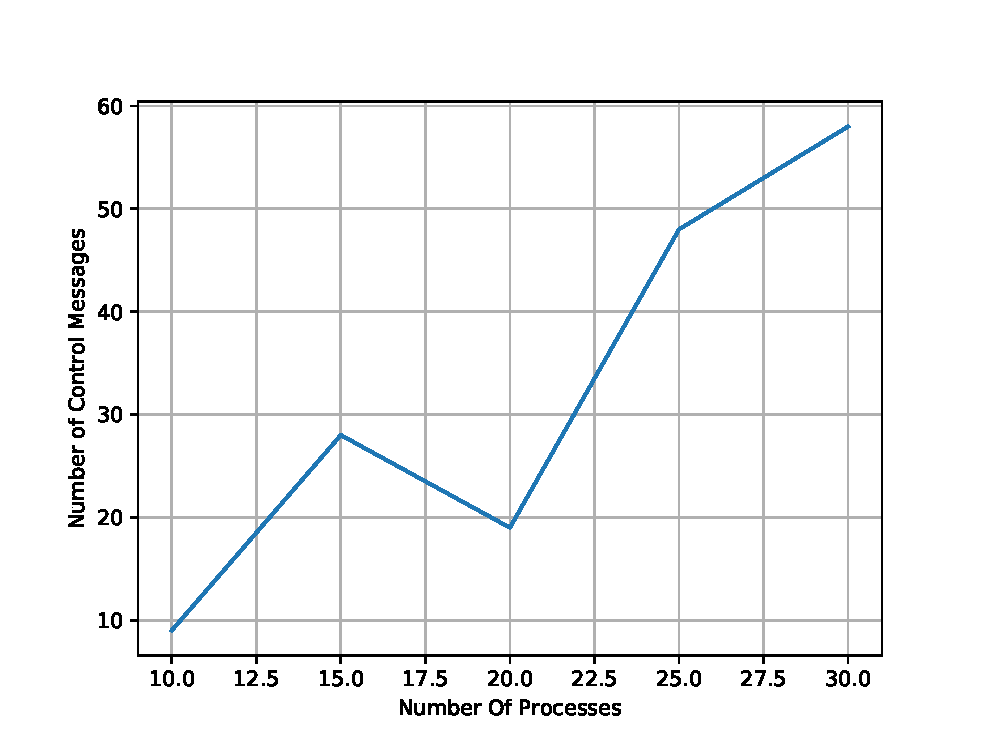
\includegraphics[scale=0.7]{./ncm1.eps}
\end{center}
\begin{center}
\begin{large}
\textbf{Number of Processes Vs Time Taken}\\
\end{large}
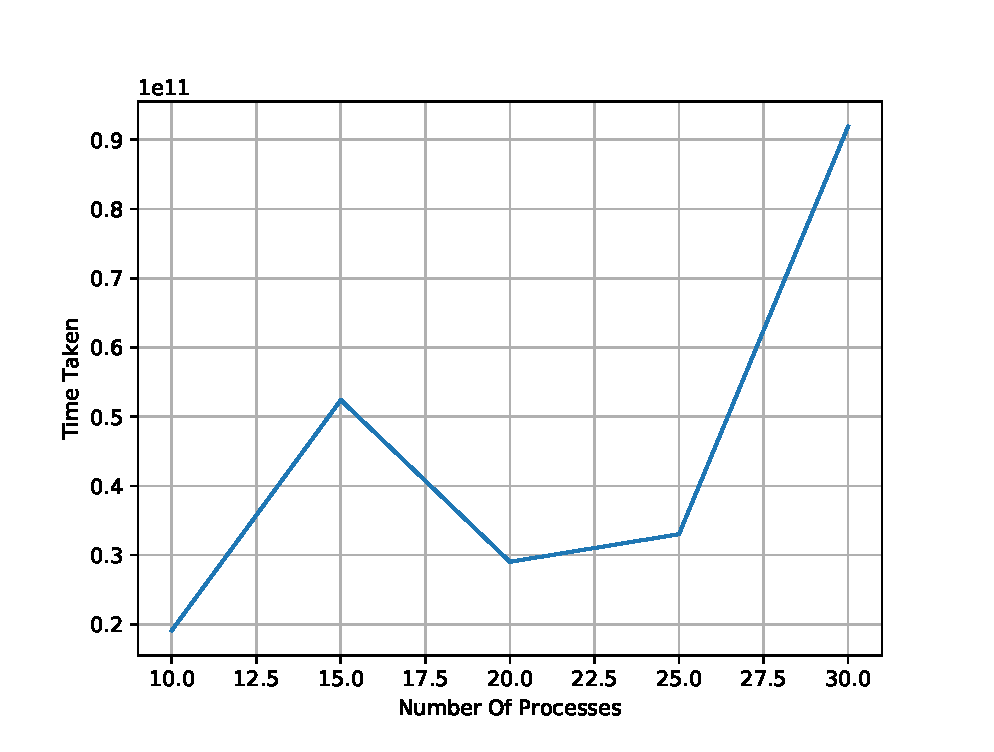
\includegraphics[scale=0.7]{./tt1.eps}
\end{center}
\subsubsection{Explaination of Results}
The following are a few points to note / observations about the above graphs:
\begin{enumerate}
\item As the number of processes increase wee notice that the number of control messages increase, this happens as more number of tokens need to be sent up the spanning tree to the root for the root to detect the termination, the graph is not purely monotonic since at times due to red cells spreading more, there are a lot of black tokens in the tree which makes the whole process repeat, so the number of control messages increases.
\item The time taken is once again expected to increase when we increase the number of processes as more messages need to be passed up the tree. Also message delays, restarting of the algorithm incase of black nodes, and other random factors like the spread of red nodes also affects the time graph.
\item Here we see that one can neither predict the time or the number of messages required for detection of the termination. The only thing we can tell for sure is that the number of messages passed would be a multiple of (N-1), since that is the number of edges in the spanning tree.
\end{enumerate}
\newpage
\subsection{Spanning Tree Algorithm}
\begin{center}
\begin{large}
\textbf{Number of Processes Vs Number of Control Message}\\
\end{large}
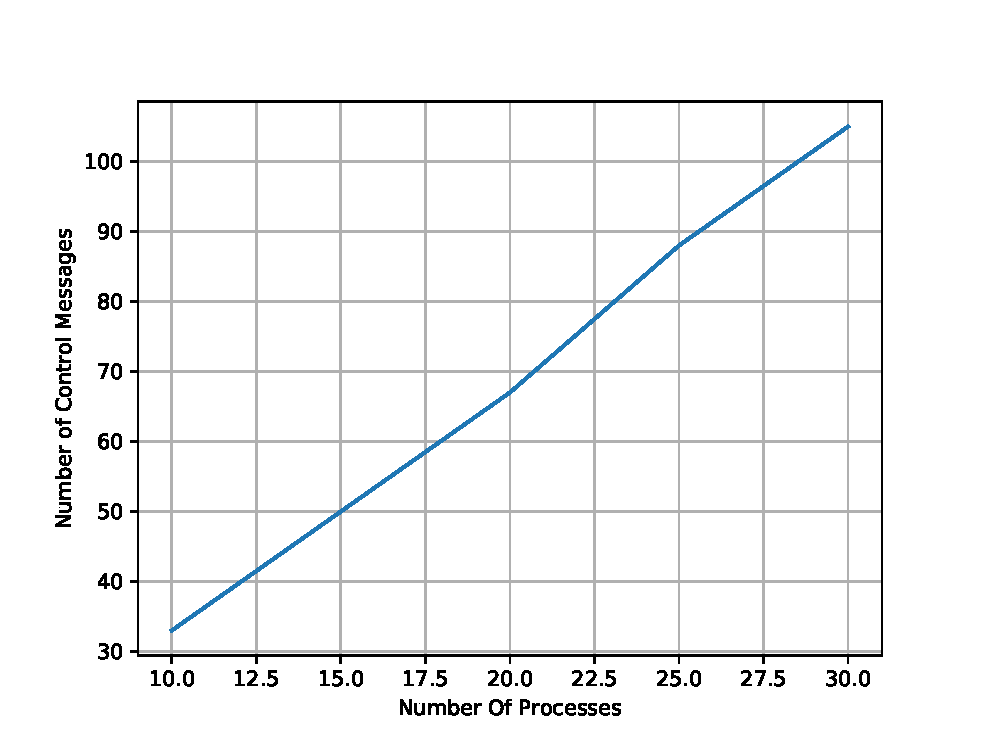
\includegraphics[scale=0.7]{./ncm2.eps}
\end{center}
\begin{center}
\begin{large}
\textbf{Number of Processes Vs Time Taken}\\
\end{large}
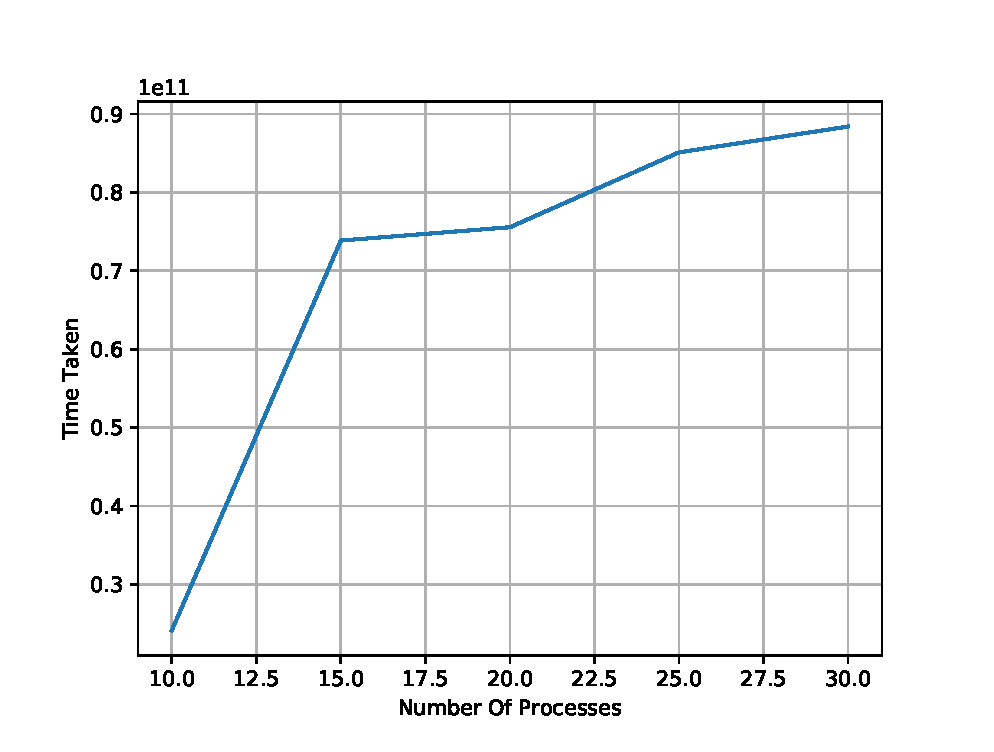
\includegraphics[scale=0.7]{./tt2.eps}
\end{center}
\subsubsection{Explaination of Results}
The following are a few points to note / observations about the above graphs:
\begin{enumerate}
\item As the number of processes increase wee notice that the number of control messages increase, this happens as more number of warning messages increases, number of terminate messages increases and the probability of number of terminate messages increasing is also high. We can also see that the number of control messages are always $\geq 3*N$, this is because there are $2*E$ warning messages and $N-1$ terminate messages and $E \geq N-1 \because\: connected\:graph$.
\item The time, as expected increases with increase in the number of cells, as the time taken to send all warning messages increases, the time taken to send terminate messages up the tree increases and also the time taken for stack cleanup also increases.
\item Compared to the spanning tree token algorithm this algorithm seems to send more control messages and take more time for the same value of N, this is because the N we have considered is small, and asymptotically this algorithm has an effecient bound.
\end{enumerate}
\end{document}